
\addtocontents{toc}{\vspace{\baselineskip}APPENDICES}

\GrizzAppendix{Statistical Summary Tables and Figures} \label{ch:extra}


\begin{figure}[!ht]
\scalebox{1.14}{
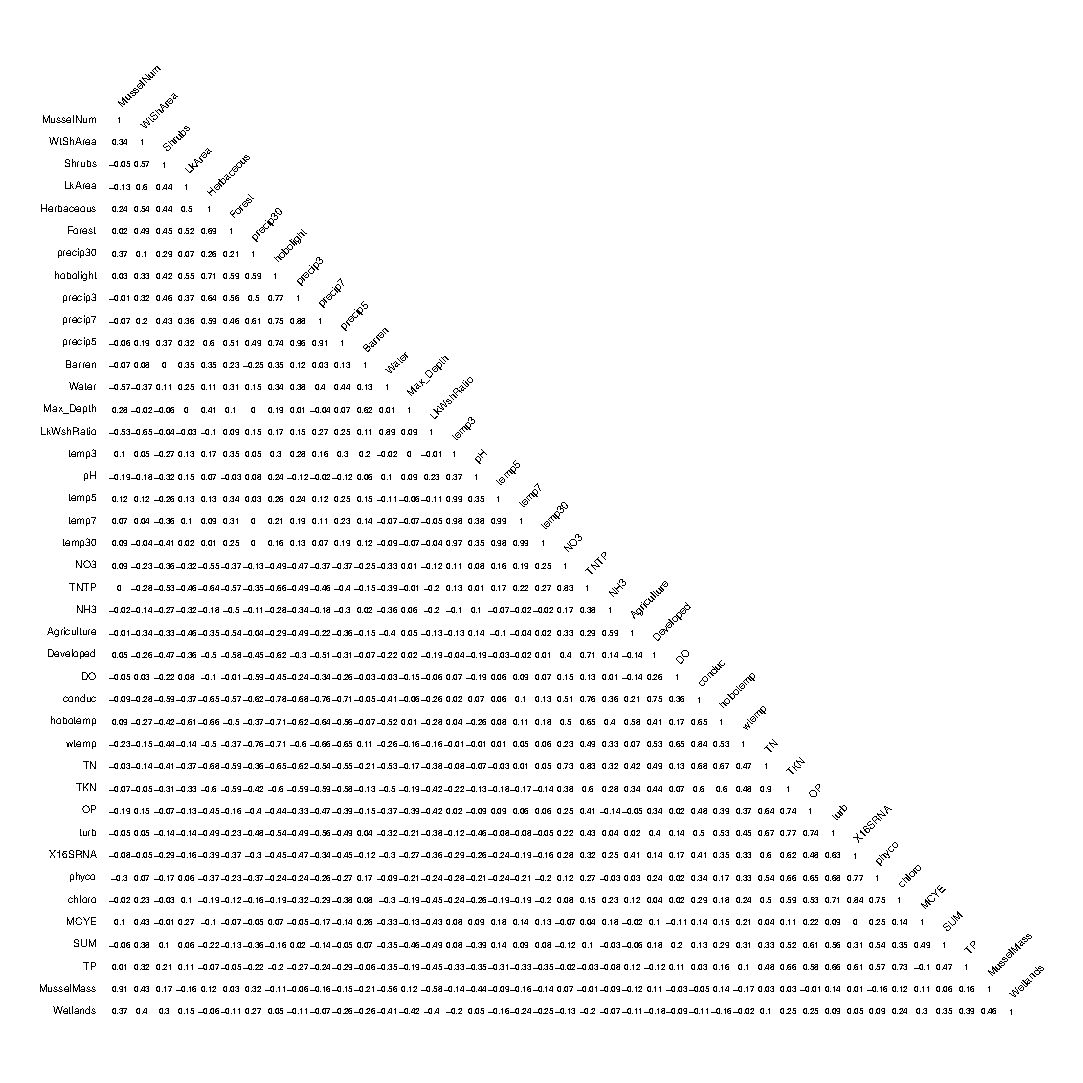
\includegraphics[width=\textwidth]{figures/matrixfull}}
\caption{Correlation matrix displaying Pearson's coefficient on the full data.}
\label{fig:matrixfull}
\end{figure}








\begin{table}[!ht]
\centering
  \caption{Microcystin congener statistical summary}
  \label{}
\begin{tabular}{@{\extracolsep{5pt}}lccccc}
\\[-1.8ex]\hline
\hline \\[-1.8ex]
Statistic & \multicolumn{1}{c}{N} & \multicolumn{1}{c}{Mean} & \multicolumn{1}{c}{St. Dev.} & \multicolumn{1}{c}{Min} & \multicolumn{1}{c}{Max} \\
\hline \\[-1.8ex]
Nodularin & 114 & 0.0003 & 0.002 & ND & 0.021 \\
{[D-Asp3]}MC-RR & 114 & 0.006 & 0.028 & ND & 0.255 \\
MC-RR & 114 & 0.185 & 0.855 & ND & 8.552 \\
MC-YR & 114 & 0.046 & 0.202 & ND & 1.799 \\
MC-HtyR & 114 & 0.002 & 0.012 & ND & 0.107 \\
MC-LR & 114 & 0.142 & 0.447 & ND & 3.570 \\
{[D-Asp3]}MC-LR & 114 & 0.027 & 0.107 & ND & 0.902 \\
MC-HilR & 114 & 0.004 & 0.019 & ND & 0.150 \\
MC-WR & 114 & 0.005 & 0.029 & ND & 0.302 \\
MC-LA & 114 & 0.088 & 0.196 & ND & 1.729 \\
MC-LY & 114 & 0.0004 & 0.002 & ND & 0.024 \\
MC-LW & 114 & ND & ND & ND & ND \\
MC-LF & 114 & 0.0002 & 0.001 & ND & 0.012 \\
MC Sum from LC MS/MS  & 114 & 0.505 & 1.580 & ND & 14.857 \\
MC from ELISA & 115 & 0.747 & 1.784 & ND & 15.320 \\
\hline \\[-1.8ex]
\multicolumn{6}{r}{Values are expressed as($\mu$g of MC*${L^{-1}}$)} \\
\multicolumn{6}{r}{ND=No Detects} \\
\end{tabular}
\end{table}

%congnenr plot by latitiude
\begin{figure}[!ht]
  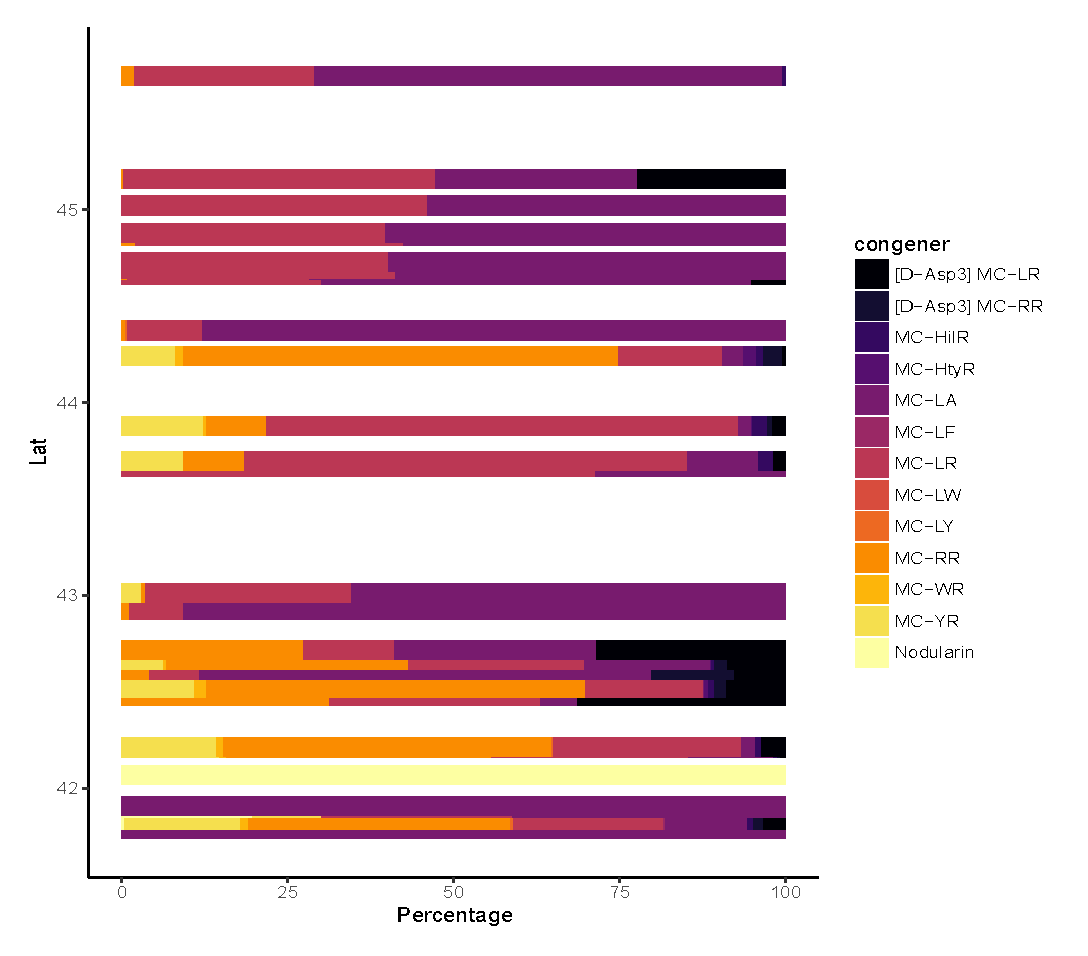
\includegraphics[width=\textwidth]{congeners}
    \caption{Proportion of MC congeners plotted by latitude}
  \label{congenerlat}
\end{figure}

\begin{table}[!ht]
  \centering
  \caption{QPCR statistical summary table}
  \label{QPCR}
  \begin{tabular}{@{\extracolsep{5pt}}lccccc}
  \\[-1.8ex]\hline
  \hline \\[-1.8ex]
  Statistic & \multicolumn{1}{c}{N} & \multicolumn{1}{c}{Mean} & \multicolumn{1}{c}{St. Dev.} & \multicolumn{1}{c}{Min} & \multicolumn{1}{c}{Max} \\
  \hline \\[-1.8ex]
  16S rRNA & 112 & 405,761 & 798,946 & ND & 6,765,631 \\
  mcyE & 91 & 8,517 & 49,396 & ND & 467,174 \\
  cyrA & 93 & ND & ND & ND & ND \\
  sxtA & 93 & ND & ND & ND & ND \\
  \hline \\[-1.8ex]
  \multicolumn{6}{r}{Values are expressed as Gene copies/mL} \\
  \multicolumn{6}{r}{ND=No Detects} \\
  \end{tabular}
  \end{table}

  \begin{figure}[!hp]
  \centering
    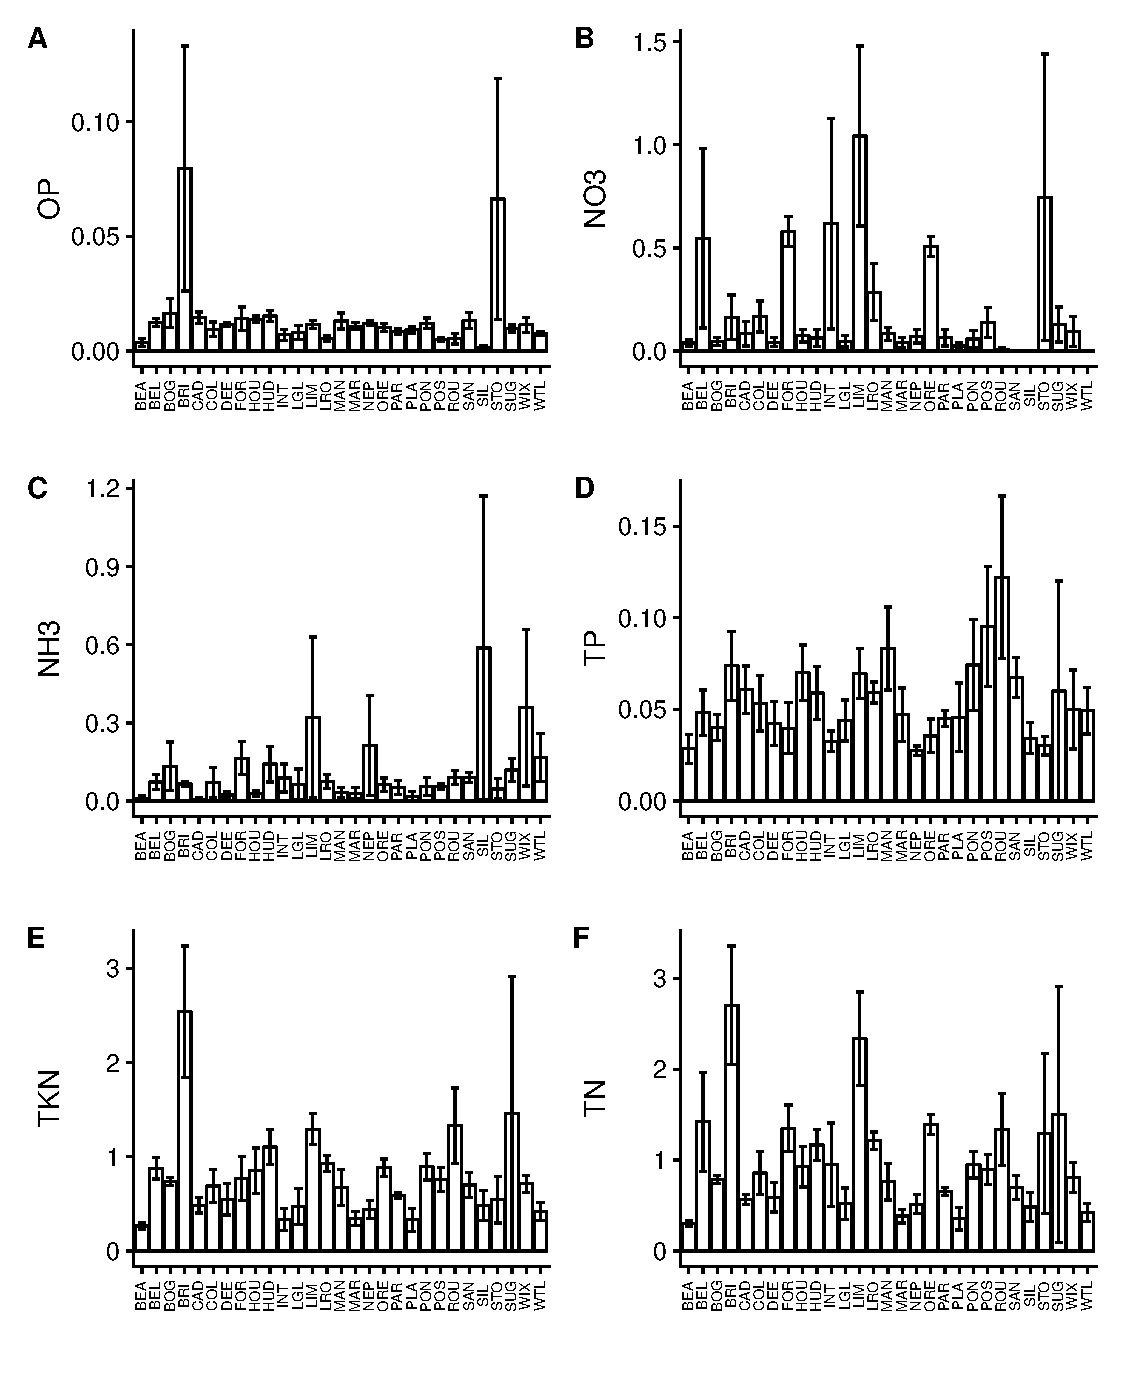
\includegraphics[width=\textwidth]{figures/nutboxplotlake}
    \caption{Average nutrient concentrations for each lake. Orthophosphate (mg-P/L) in figure (A), nitrate+nitrite (mg-N/L) in figure (B), ammonia (mg-N/L) in figure (C), total phosphorus (mg-P/L) in figure (D) and total Kjeldahl nitrogen (mg-N/L) in figure (E). Error bars represents one standard deviation of the mean. }
    \label{fig:nutrients}
  \end{figure}


  \begin{table}[!ht]
    \centering
    \caption{Lake nutrients statistical summary}
    \label{}
  \begin{tabular}{@{\extracolsep{5pt}}lccccc}
  \\[-1.8ex]\hline
  \hline \\[-1.8ex]
  Statistic & \multicolumn{1}{c}{N} & \multicolumn{1}{c}{Mean} & \multicolumn{1}{c}{St. Dev.} & \multicolumn{1}{c}{Min} & \multicolumn{1}{c}{Max} \\
  \hline \\[-1.8ex]
   Orthophosphate (mg P/L) & 114 & 0.015 & 0.030 & ND & 0.237 \\
  Nitrate+Nitrite (mg N/L) & 115 & 0.199 & 0.443 & ND & 2.827 \\
  Ammonia (mg N/L)  & 115 & 0.112 & 0.281 & ND & 2.338 \\
  Total Phosphorus (mg P/L) & 114 & 0.055 & 0.037 & ND & 0.239 \\
  Total Kjeldahl Nitrogen (mg N/L) & 114 & 0.763 & 0.602 & ND & 4.555 \\
  Total Nitrogen & 114 & 1.074 & 0.870 & 0.103 & 4.717 \\
  \hline \\[-1.8ex]
  \multicolumn{6}{r}{ND=No Detects} \\
  \end{tabular}
  \end{table}

  \begin{figure}[!hp]
  \centering
    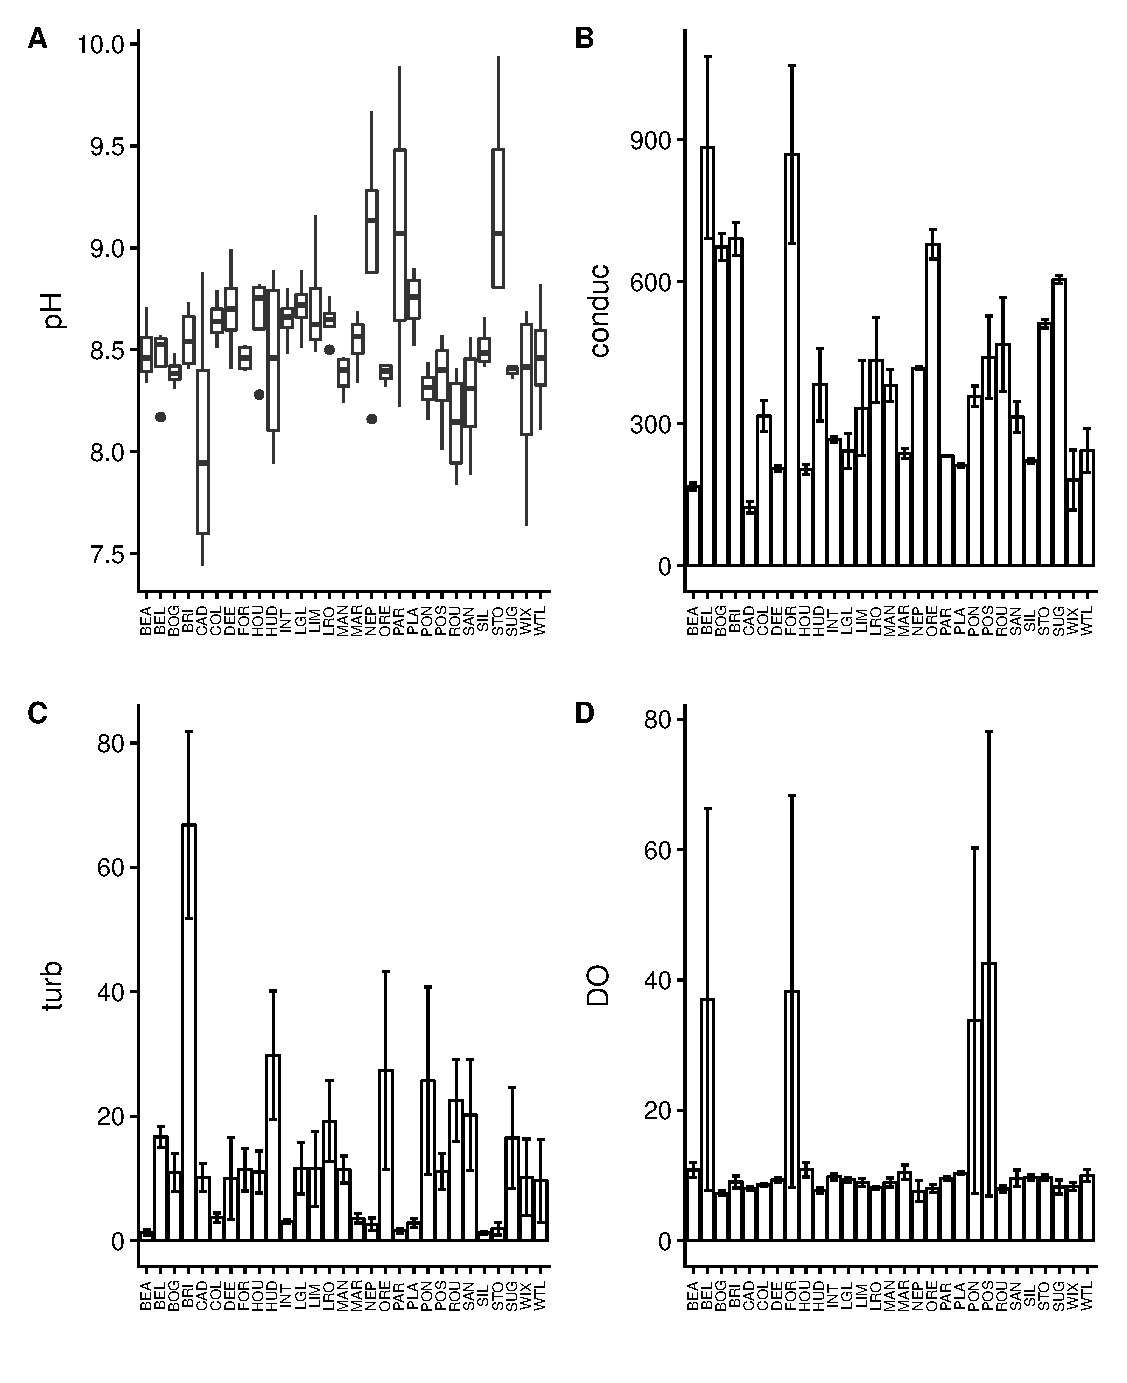
\includegraphics[width=\textwidth]{figures/watboxplotlake.eps}
    \caption{Summary of measured water chemical parameters: A box and whisker plot of pH in figure (A). Bar plots of average conductance (B), average turbidity (C), and average dissolved oxygen (D) plotted by each lake. }
  \end{figure}
